% Digital Logic Report Template
% Created: 2020-01-10, John Miller

%==========================================================
%=========== Document Setup  ==============================

% Formatting defined by class file
\documentclass[11pt]{article}

% ---- Document formatting ----
\usepackage[margin=1in]{geometry}	% Narrower margins
\usepackage{booktabs}				% Nice formatting of tables
\usepackage{graphicx}				% Ability to include graphics

%\setlength\parindent{0pt}	% Do not indent first line of paragraphs 
\usepackage[parfill]{parskip}		% Line space b/w paragraphs
%	parfill option prevents last line of pgrph from being fully justified

% Parskip package adds too much space around titles, fix with this
\RequirePackage{titlesec}
\titlespacing\section{0pt}{8pt plus 4pt minus 2pt}{3pt plus 2pt minus 2pt}
\titlespacing\subsection{0pt}{4pt plus 4pt minus 2pt}{-2pt plus 2pt minus 2pt}
\titlespacing\subsubsection{0pt}{2pt plus 4pt minus 2pt}{-6pt plus 2pt minus 2pt}

% ---- Hyperlinks ----
\usepackage[colorlinks=true,urlcolor=blue]{hyperref}	% For URL's. Automatically links internal references.

% ---- Code listings ----
\usepackage{listings} 					% Nice code layout and inclusion
\usepackage[usenames,dvipsnames]{xcolor}	% Colors (needs to be defined before using colors)

% Define custom colors for listings
\definecolor{listinggray}{gray}{0.98}		% Listings background color
\definecolor{rulegray}{gray}{0.7}			% Listings rule/frame color

% Style for Verilog
\lstdefinestyle{Verilog}{
	language=Verilog,					% Verilog
	backgroundcolor=\color{listinggray},	% light gray background
	rulecolor=\color{blue}, 			% blue frame lines
	frame=tb,							% lines above & below
	linewidth=\columnwidth, 			% set line width
	basicstyle=\small\ttfamily,	% basic font style that is used for the code	
	breaklines=true, 					% allow breaking across columns/pages
	tabsize=3,							% set tab size
	commentstyle=\color{gray},	% comments in italic 
	stringstyle=\upshape,				% strings are printed in normal font
	showspaces=false,					% don't underscore spaces
}

% How to use: \Verilog[listing_options]{file}
\newcommand{\Verilog}[2][]{%
	\lstinputlisting[style=Verilog,#1]{#2}
}

\usepackage[section]{placeins}



%======================================================
%=========== Body  ====================================
\begin{document}

\title{ELC 2137 Lab 5: Intro to Verilog}
\author{Aaron Mendoza}

\maketitle


\section*{Summary}

The purpose of this lab is to familiarize myself with Verilog coding by building a half adder, full adder, and 2 bit adder/subtractor on Vivado. 

There are three different types of coding styles: gate-level, functional/behavioral, and structural. Gate-level coding utilizes the actual gates within the code. This is done by literally typing out the exact gate like "xor" within the code. Behavioral coding is different from gate-level because the gate is not actually specified, but rather the behavior of the gate is achieved through the code that is written. This utilizes symbols like the ampersand. Structural coding is code that works based off of other code that has already been previously written. For example, the full adder code uses the half adder code within it. 

I used behavorial coding when building my half adder, full adder, and 2 bit adder/subtractor. I used structural coding to build my full adder and my 2 bit adder/subtractor.


\subsection*{Block Diagrams}
\begin{figure}[ht]\centering
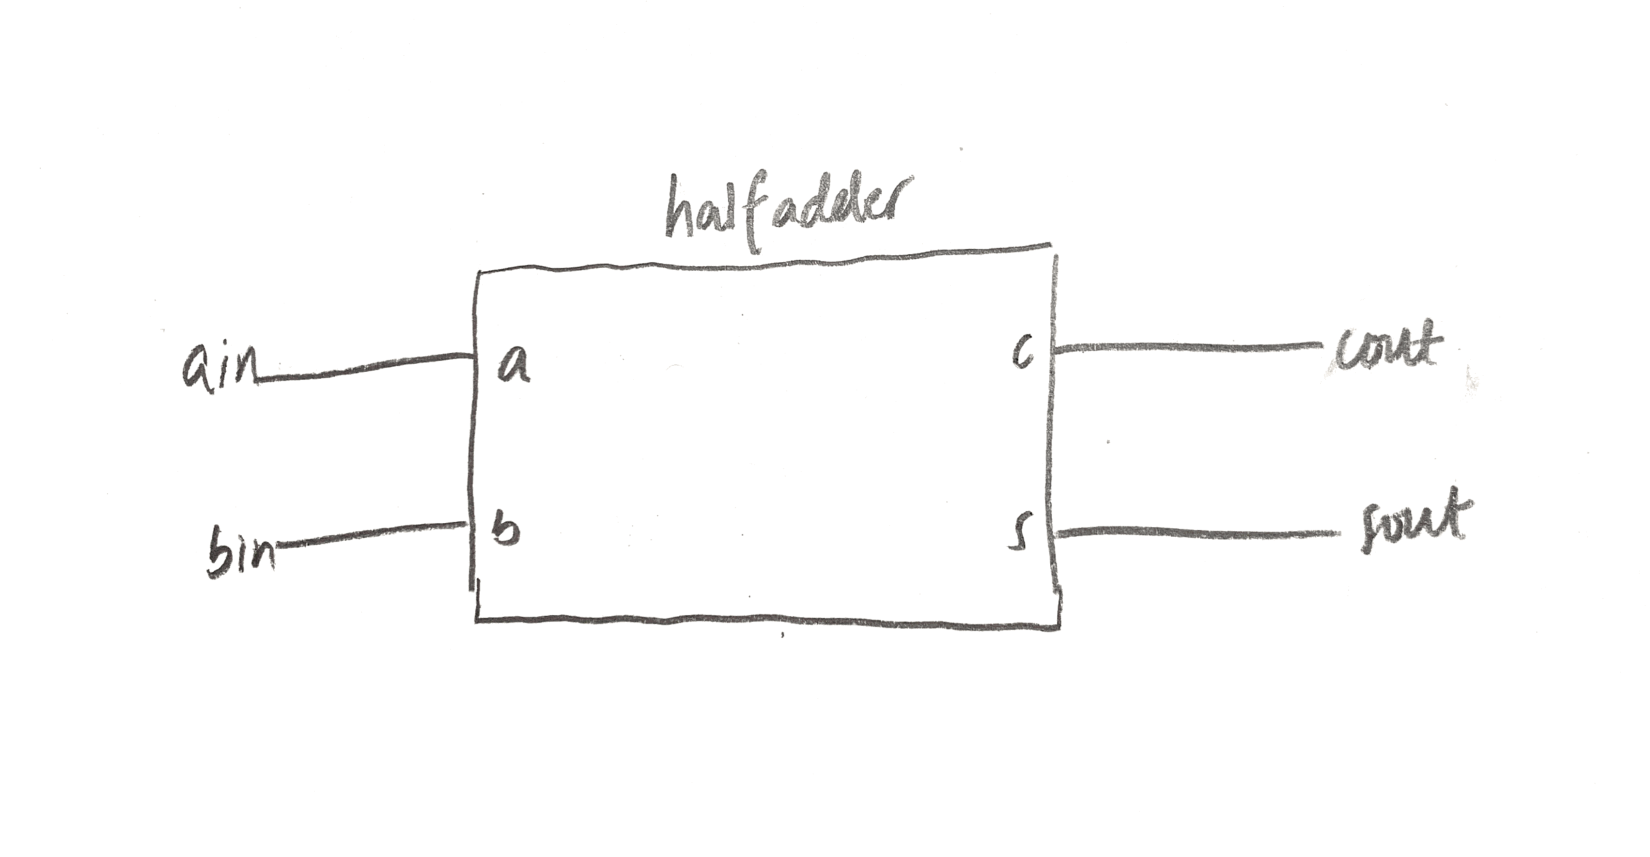
\includegraphics[width=0.5\textwidth]{lab05_halfadder_block}
\caption{This is the block diagram for a half adder.}
\label{fig:original_logo}
\end{figure}
\begin{figure}[ht]\centering
	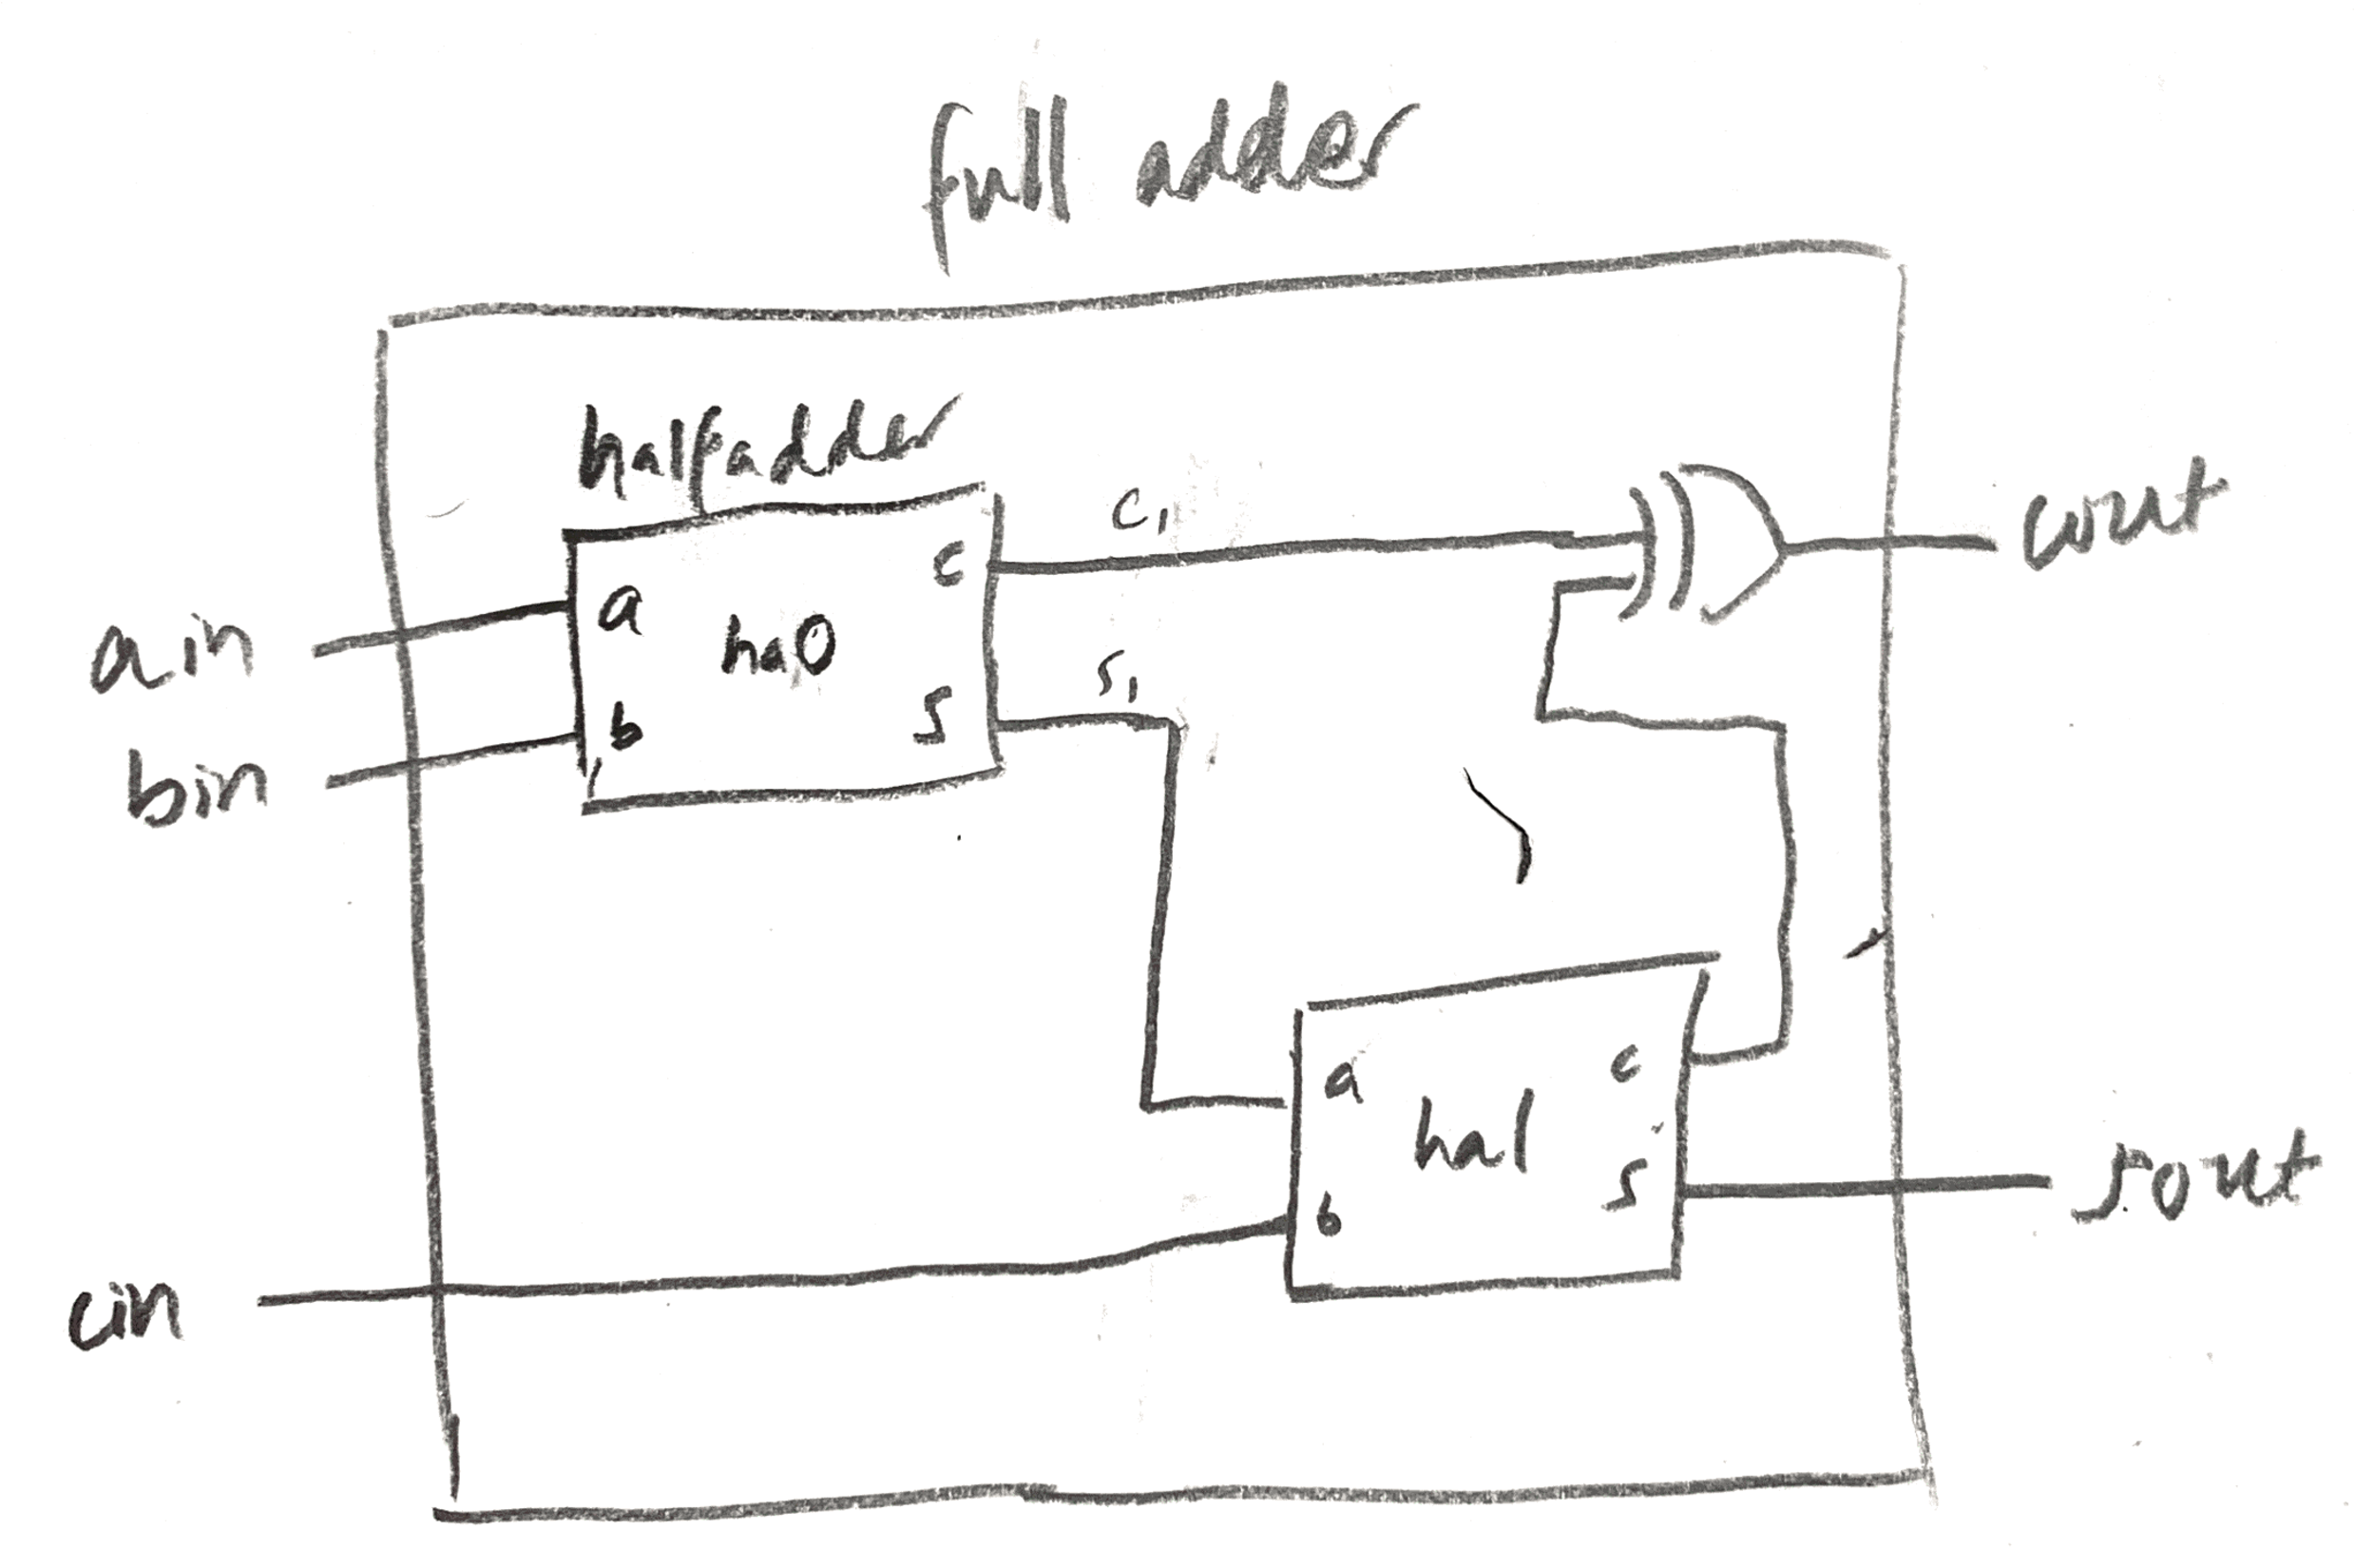
\includegraphics[width=0.5\textwidth]{lab05_fulladder_block}
	\caption{This is the block diagram for a full adder.}
	\label{fig:original_logo}
\end{figure}
\begin{figure}[ht]\centering
	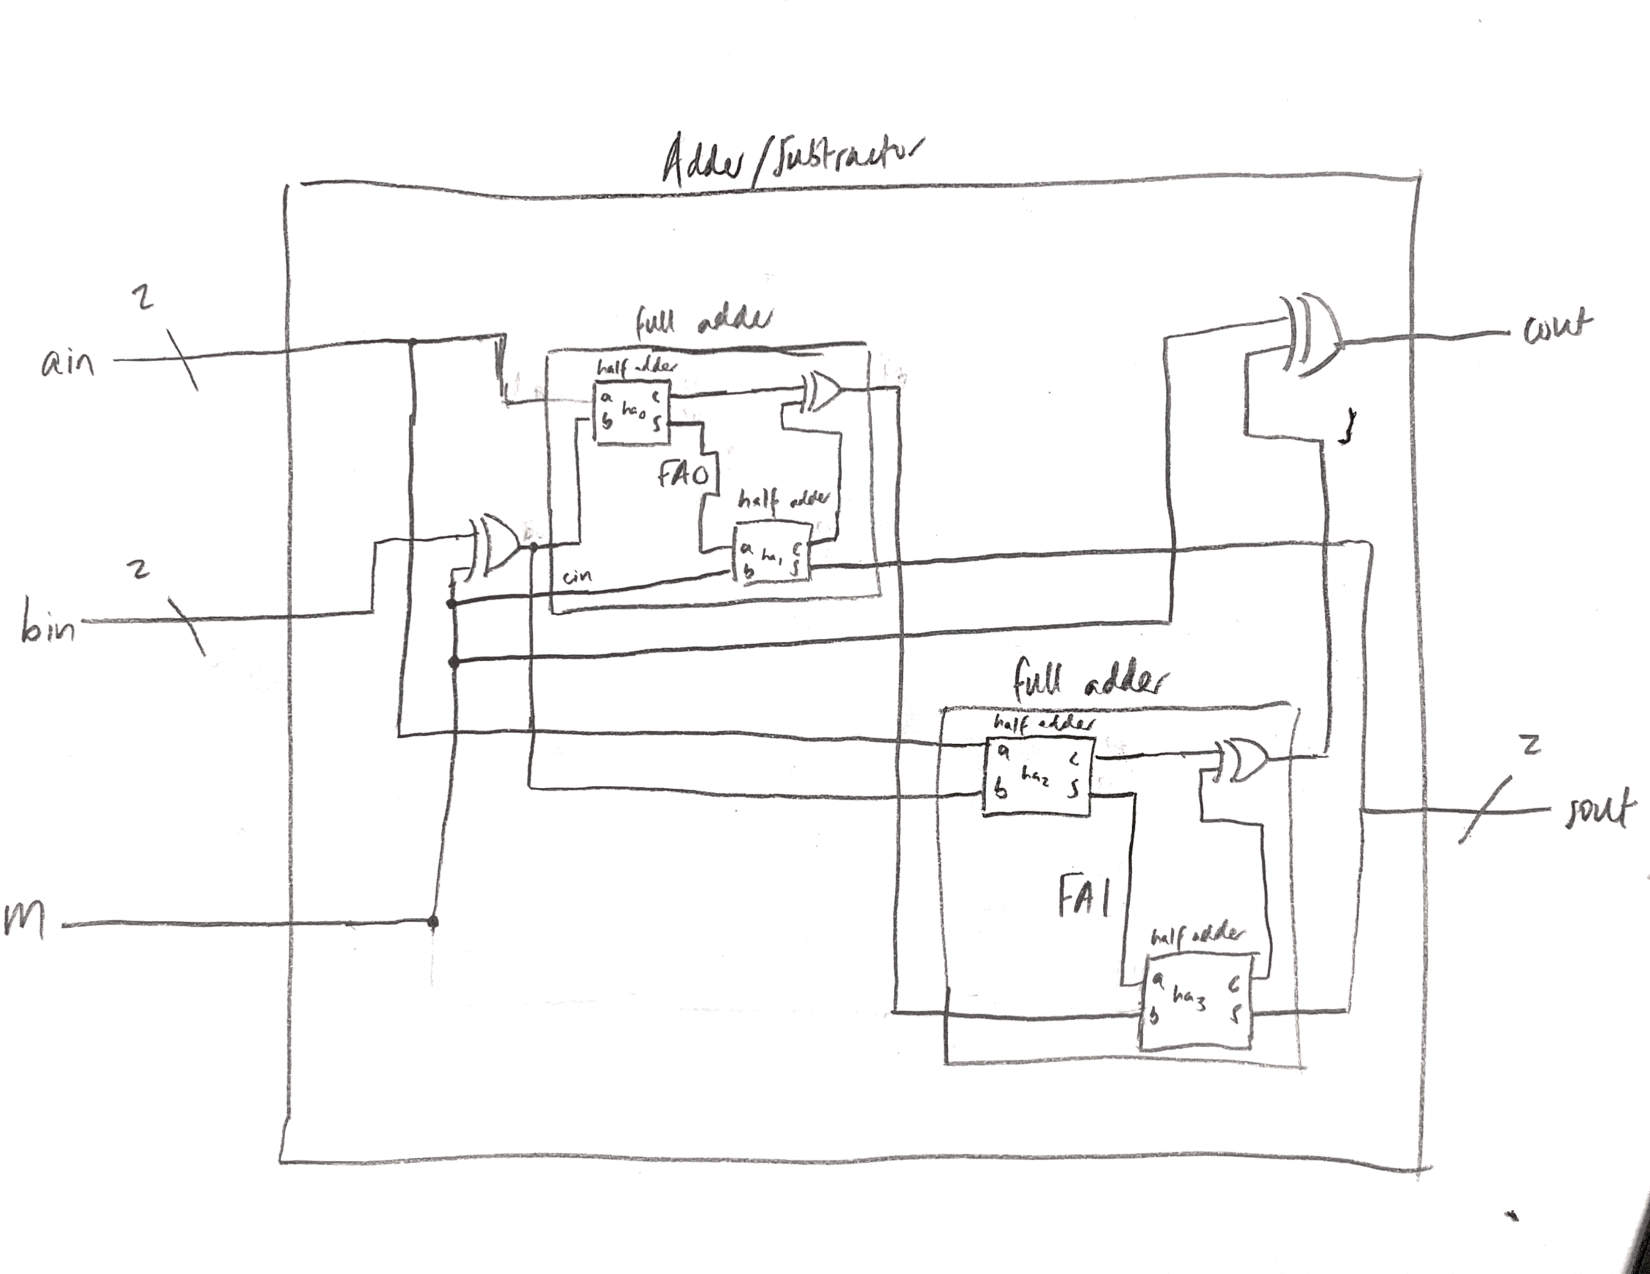
\includegraphics[width=0.9\textwidth]{lab05_addsub_block}
	\caption{This is the block diagram for an adder/subtractor.}
	\label{fig:original_logo}
\end{figure}

\FloatBarrier
\section*{Q\&A}

\begin{enumerate}
	\item Do the simulations match the expected output values?
		
		Yes the simulations match the expected output values.
		
	\item What is one thing that you still don't understand about Verilog?
	
		I still don't completely understand the "always" block.
		
\end{enumerate}


\section*{Results}

\begin{figure}[ht]\centering
	\begin{tabular}{l|rrrr}
		Time (ns): & 0 & 10 & 20 & 30 \\
		\midrule
		a & 0 & 0 & 1 & 1 \\
		b & 0 & 1 & 0 & 1 \\
		\midrule
		c & 0 & 0 & 0 & 1 \\
		s & 0 & 1 & 1 & 0 \\
		\bottomrule
	\end{tabular}\medskip
	
	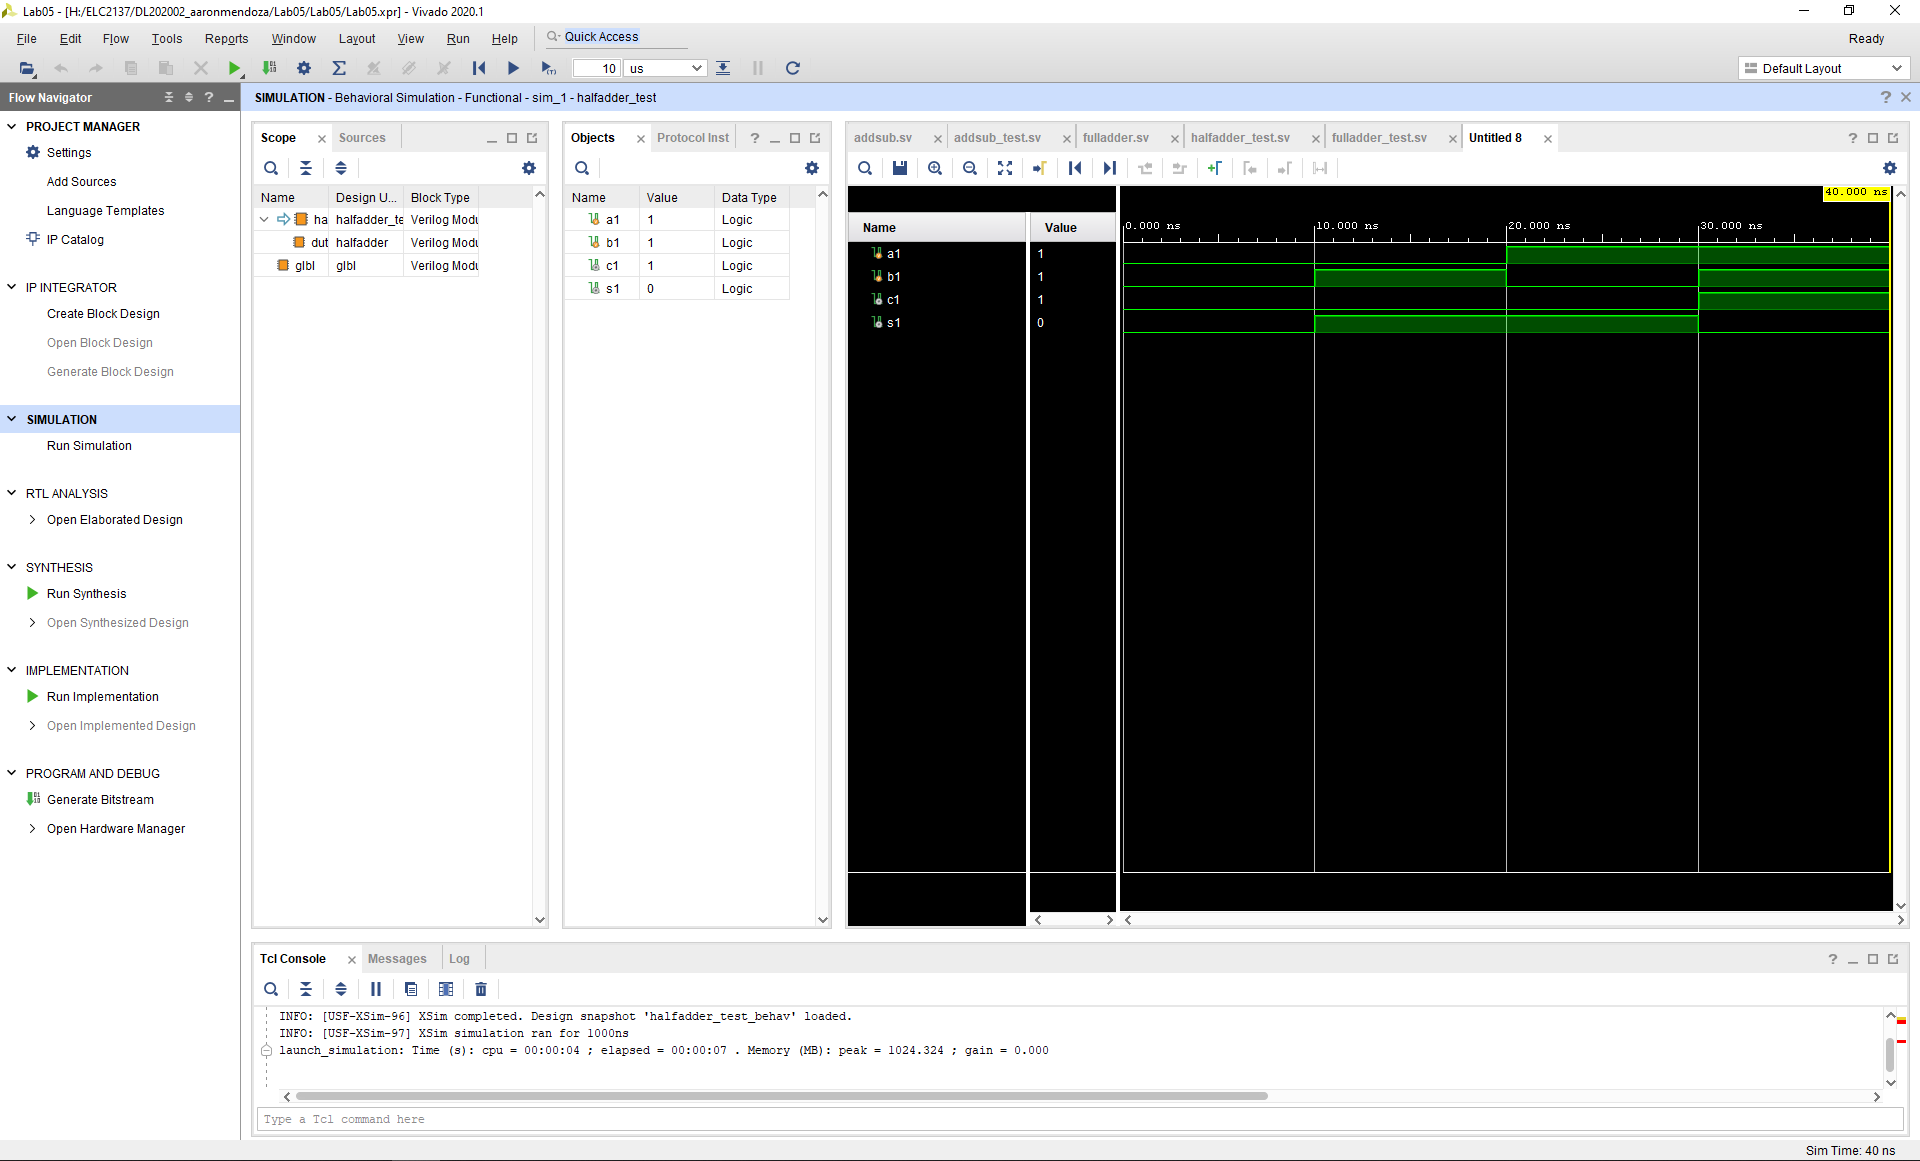
\includegraphics[width=1\textwidth,trim=19cm 15cm 0.5cm 4.5cm,clip]{lab05_halfadder_screenshot}
	\caption{Half adder simulation waveform and ERT}
	\label{fig:sim_with_table}
\end{figure}

\begin{figure}[ht]\centering
	\begin{tabular}{l|rrrrrrrr}
		Time (ns): & 0 & 10 & 20 & 30 & 40 & 50 & 60 & 70 \\
		\midrule
		a & 0 & 0 & 0 & 0 & 1 & 1 & 1 & 1 \\
		b & 0 & 0 & 1 & 1 & 0 & 0 & 1 & 1 \\
		cin & 0 & 1 & 0 & 1 & 0 & 1 & 0 & 1 \\
		\midrule
		cout & 0 & 0 & 0 & 1 & 0 & 1 & 1 & 1 \\
		sout & 0 & 1 & 1 & 0 & 1 & 0 & 0 & 1 \\
		\bottomrule
	\end{tabular}\medskip
	
	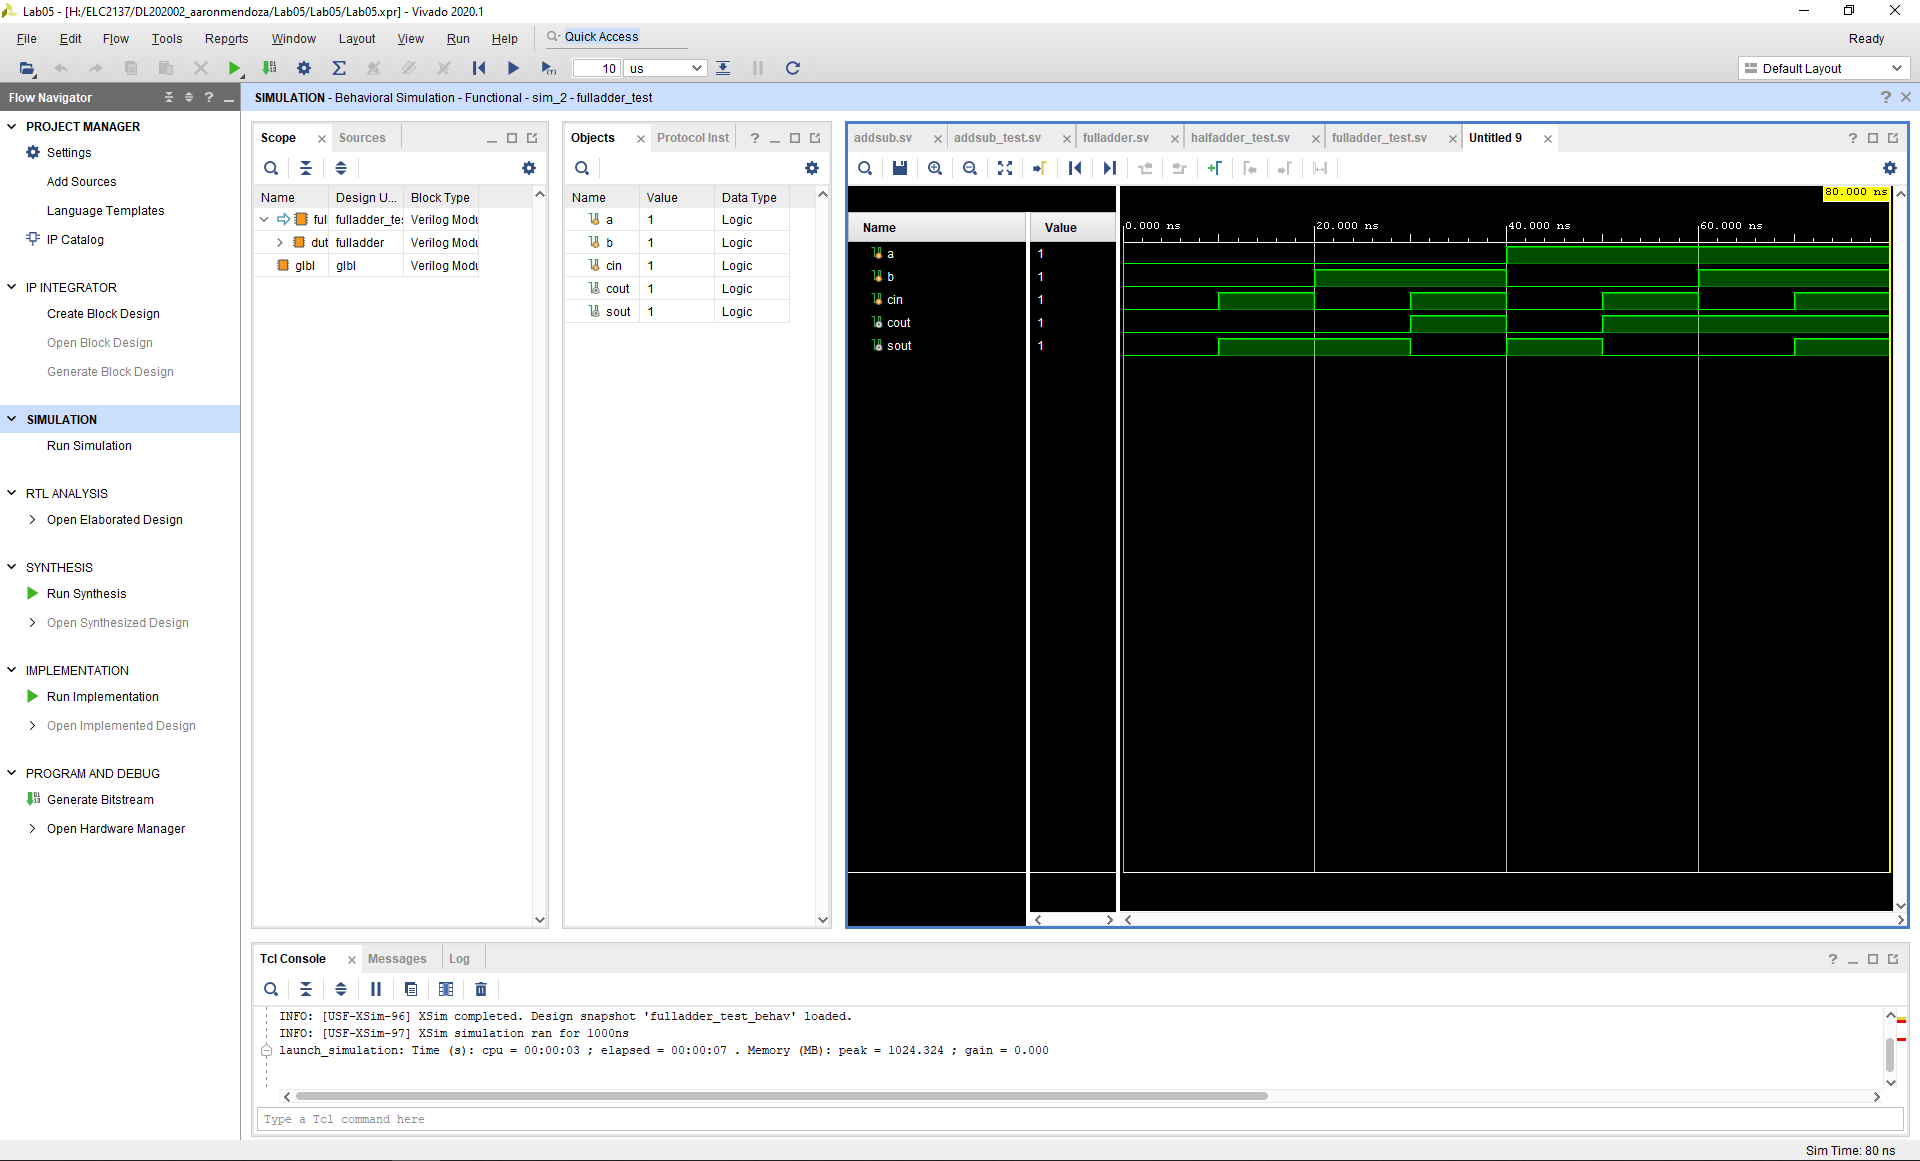
\includegraphics[width=1\textwidth,trim=19cm 15cm 0.5cm 4.5cm,clip]{lab05_fulladder_screenshot}
	\caption{Full adder simulation waveform and ERT}
	\label{fig:sim_with_table}
\end{figure}

\begin{figure}[ht]\centering
	\begin{tabular}{l|rrrrrrrrrrrrrrrrrrrrrrrrrrrrrrrr}
		Time (ns): & 0 & 10 & 20 & 30 & 40 & 50 & 60 & 70 & 80 & 90 & 100 & 110 & 120 & 130 & 140 & 150 & 160 & 170 & 180 & 190 & 200 & 210 & 220 & 230 & 240 & 250 & 260 & 270 & 280 & 290 & 300 & 310 \\
		\midrule
		a & 0 & 0 & 0 & 0 & 0 & 1 & 1 & 1 & 0 & 0 & 0 & 0 & 1 & 1 & 1 & 1 & 0 & 0 & 0 & 0 & 1 & 1 & 1 & 1 & 0 & 0 & 0 & 0 & 1 & 1 & 1 & 1 \\
		b & 0 & 0 & 1 & 1 & 0 & 0 & 1 & 1 \\
		m & 0 & 1 & 0 & 1 & 0 & 1 & 0 & 1 \\
		\midrule
		cout & 0 & 0 & 0 & 1 & 0 & 1 & 1 & 1 \\
		sout & 0 & 1 & 1 & 0 & 1 & 0 & 0 & 1 \\
		\bottomrule
	\end{tabular}\medskip
	
	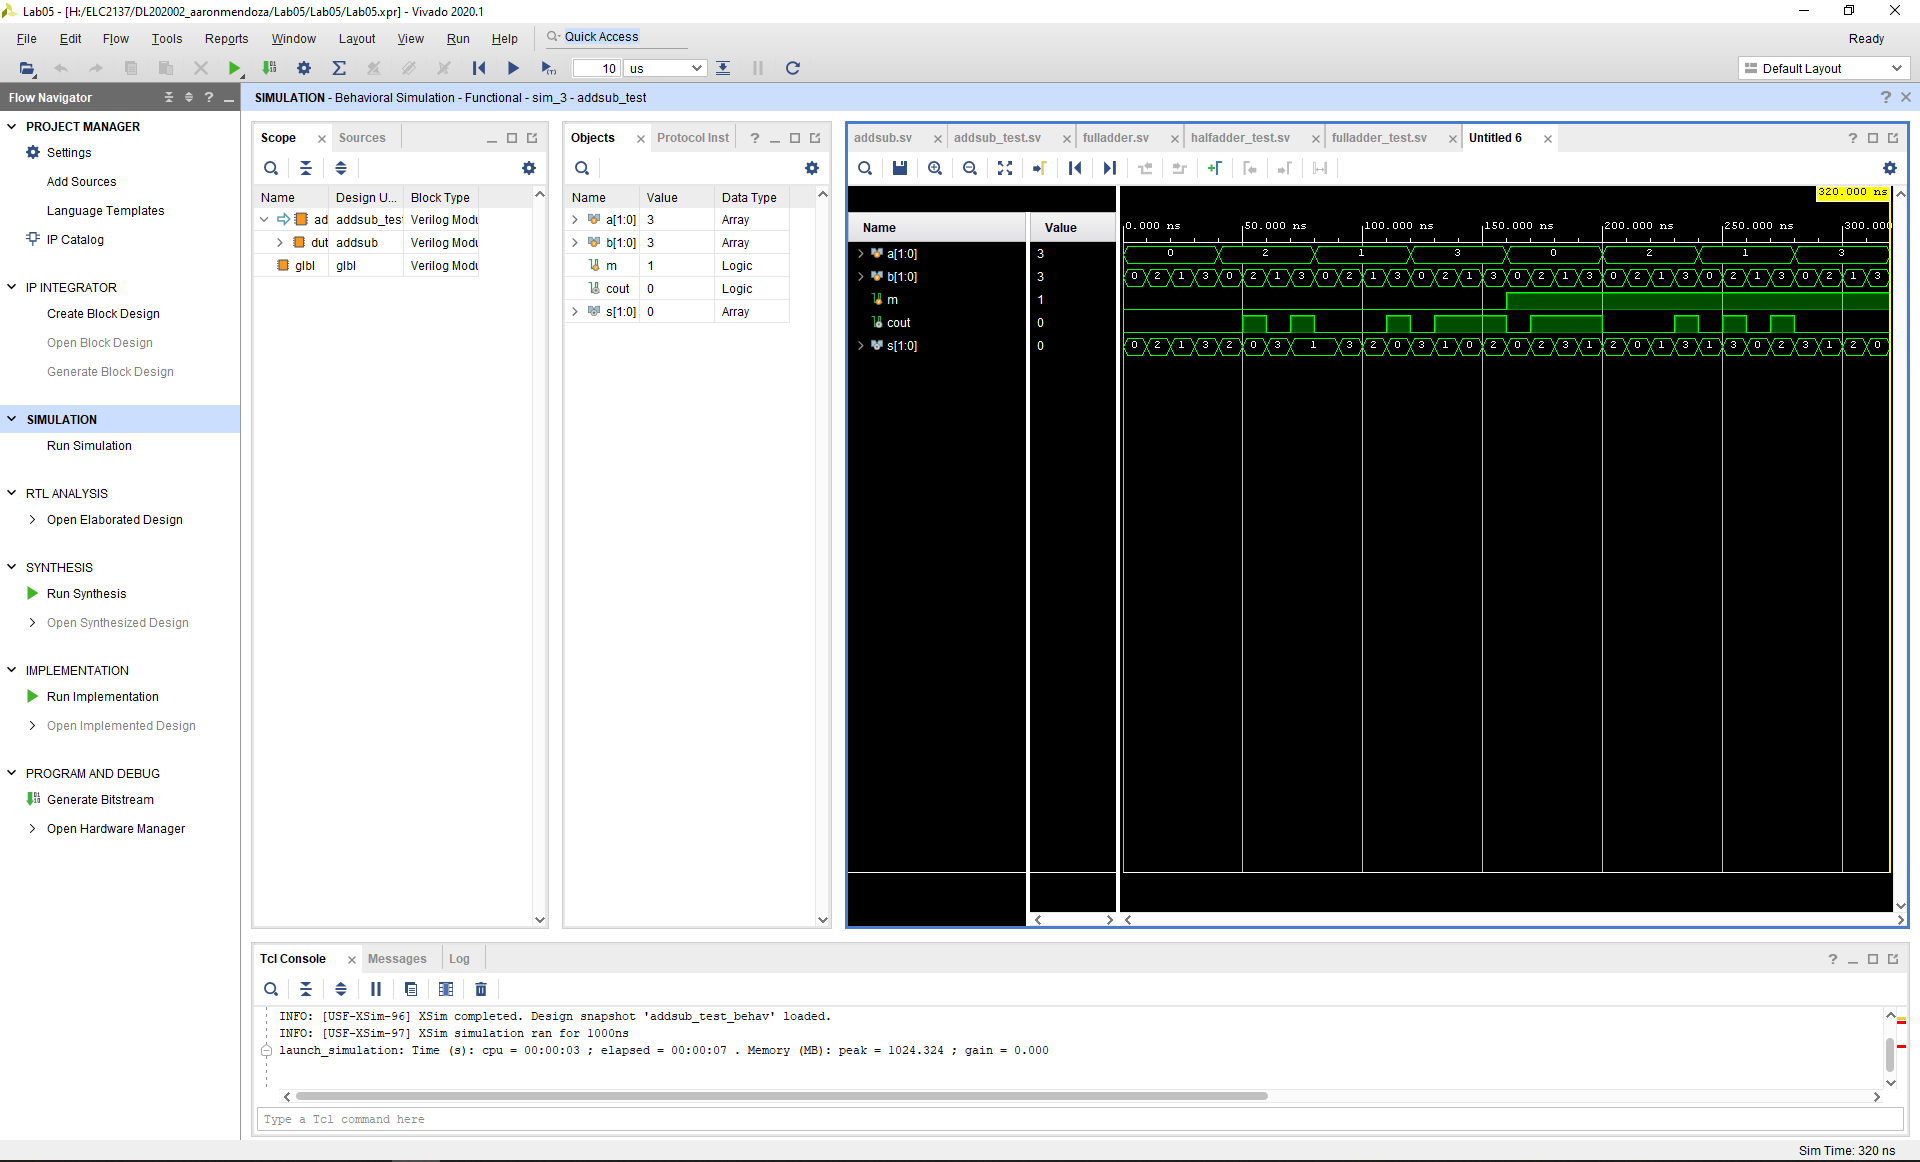
\includegraphics[width=1\textwidth,trim=19cm 15cm 0.5cm 4.5cm,clip]{lab05_addsub_screenshot}
	\caption{Adder/Subtractor simulation waveform and ERT}
	\label{fig:sim_with_table}
\end{figure}


\section*{Code}

\Verilog[firstline=22, lastline=56, caption=Half Adder Verilog code]{Lab05/codedirectory/halfadder.sv}|

\Verilog[firstline=22, lastline=46, caption=Half Adder Test Bench Verilog code]{Lab05/codedirectory/halfadder_test.sv}|

\Verilog[firstline=22, lastline=50, caption=Full Adder Verilog code]{Lab05/codedirectory/fulladder.sv}|

\Verilog[firstline=22, lastline=51, caption=Full Adder Test Bench Verilog code]{Lab05/codedirectory/fulladder_test.sv}|

\Verilog[firstline=22, lastline=56, caption=Adder/Subtractor Verilog code]{Lab05/codedirectory/addsub.sv}|

\Verilog[firstline=22, lastline=76, caption=Adder/Subtractor Test Bench Verilog code]{Lab05/codedirectory/addsub_test.sv}|



\end{document}
